\section{Übergreifende Datenarchitektur}
\label{sec:globale-architektur}

Letztere hingegen setzt auf die regionalen Datenarchitekturen auf,
erweitert diese und führt sie Regions-übergreifend zusammen.
Die beiden komplexeren Data Science Anwendungsfälle 
sind hier nicht mehr Teil des Betrachtungsgegenstands.
Stattdessen sind die Anforderungen, die in diesem Abschnitt abgedeckt werden,
übliche BI Fragestellungen.
Einerseits regionale Anforderungen, die aus dem ersten Abschnitt 
rausgelassen werden, um den Fokus nicht von den speziellen Use Cases zu verschieben.
Und andererseits strukturierte Datenanalysen,
die für den gesamten Konzern beantwortet werden sollen.

\begin{figure}[tbh]
    \centering
    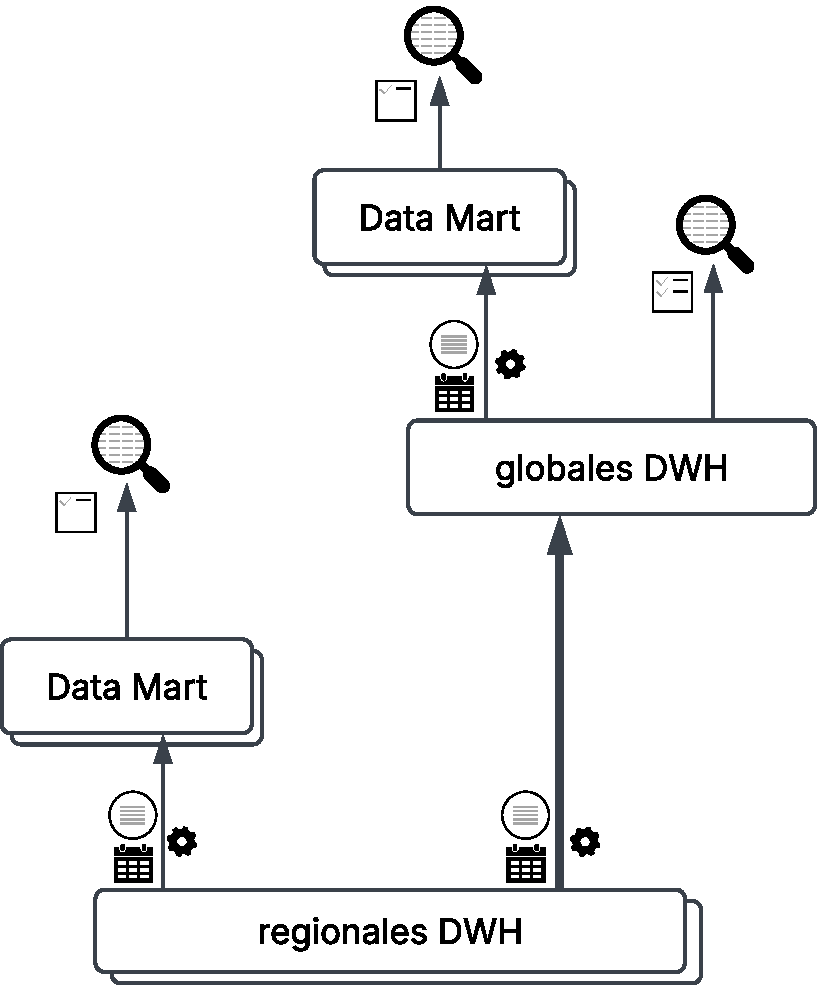
\includegraphics[width=0.5\textwidth]{images/Diagram_globale_Datenarchitektur.pdf}
    \caption{globale Datenarchitektur für BI Anwendungsfälle}\label{fig:datenarchitektur-global}
\end{figure}